%!TEX root = ./rules-working.tex
%LTeX: enabled=false

\rulechapter{Positioning Game Counters}

This chapter describes how the map hexes are utilized to position counters during play. The game map is used to show exactly where aircraft, missiles, and other units, are located in relationship to each other. Every game counter must be placed on the maps so that its position is clear to all players.


\section{Basic Elements of Position}
\label{rule:position}

\paragraph{Aircraft and Missile Counters.} 
Each aircraft and missile counter has a position which is defined by its map location, facing, and altitude.

\begin{itemize}
    \item \itemparagraph{Map Location.} With respect to the hexgrid, aircraft and missiles may be located wholly within a hex or on one of the lines between two hexes (commonly called a hexside). When located on a hexside, the game counter must face parallel to that hexside as illustrated \changedin{1B}{1B-figures}{below}{in \changedin{3A}{3A-ship-facing}{Figure~\ref{figure:map-location}}{Figure~\ref{figure:map-location-for-aircraft-and-missiles}}}. \deletedin{2B}{2B-range}{\addedin{1C}{1C-apj-23-errata}{When determining range when one or both aircraft are on hexsides, count only the full hexes between them. Take the shortest number of hexes.}}

    \item \itemparagraph{Facing.} This is the horizontal direction in which an aircraft or missile is flying. Use the silhouette on the counter to show facing by pointing the nose of the aircraft or missile in one of the twelve possible directions. Each direction differs by 30 degrees and has a corresponding compass heading associated with it (i.e., N = North, SSE = South South-East, etc.). In the scenario booklets, next to the map layout diagrams, there will be a compass arrow indicating which direction relative to the hexgrid that is North. \changedin{1B}{1B-figures}{See diagram below.}{See Figure~\ref{figure:facing}.}

    \item \itemparagraph{Altitude.} 
    An aircraft or missile's altitude is kept track of on the aircraft's log sheet in terms of numbered levels. Each altitude level represents 1000 feet of height thus the number of a level corresponds to the altitude in thousands of feet (i.e., level 24 = 24,000 feet). Altitude levels are further grouped into named bands as described later in the rules. Aircraft and missile performance may vary in each altitude band as shown on an aircraft's data card and in the missile flight tables.

\end{itemize}


\changedin{3A}{3A-ship-facing}{
\paragraph{Ground and Naval Unit Counters.}
Ground combat units and naval units have their positions defined simply by map location. They are always placed wholly within hexes and never on hexsides. Ground units never consider facing\addedin{1C}{1C-apj-23-errata}{ (except heavy AAA units under advanced rule \ref{rule:heavy-aaa-unit-facing})}, but large naval units must be faced in specific directions as for aircraft and missiles.
}{
\paragraph{Ground Unit Counters.}
Each ground unit counter has a position which is defined simply by its map location. They are always placed wholly within hexes and never on hexsides. Ground units never consider facing (except heavy AAA units under advanced rule \ref{rule:heavy-aaa-unit-facing}). See Figure~\ref{figure:map-location-for-ground-units}.

\paragraph{Ship Counters.}
Each ship counter has a position which is defined by its map location and facing. They are always placed wholly within hexes and never on hexsides. Use the silhouette on the counter to show facing by pointing the bow of the ship in one of the six possible directions towards adjacent hexes. Unlike aircraft and missiles, ships cannot face towards hexsides. See Figure~\ref{figure:map-location-for-ships}.
}

\silentlyaddedin{1B}{1B-figures}{
    \begin{tikzfigure}{0.5\linewidth}
    \drawhexgrid{5}{3}  
    \drawaircraftcounter{2.00}{2.00}{90}{F-4}{}
    \drawaircraftcounter{1.50}{0.75}{120}{F-4}{}
    \drawaircraftcounter{4.00}{1.50}{90}{F-4}{}
    \miniathex{1.00}{1.50}{\node {\scriptsize Legal};}
    \miniathex{4.00}{2.20}{\node {\scriptsize Illegal};}
\end{tikzfigure}


    \begin{fitwidth}{0.7\linewidth}
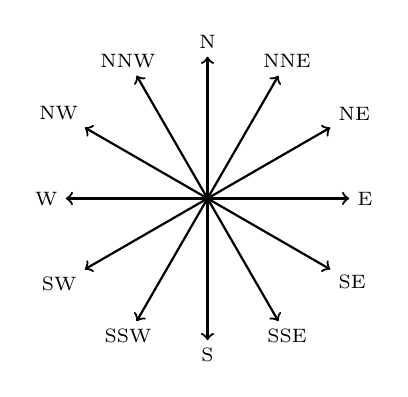
\begin{tikzpicture}
    \scriptsize
    \drawhex{0}{0}  
    \drawhex{0}{+1}  
    \drawhex{0}{-1}  
    \drawhex{+1}{+0.5}  
    \drawhex{+1}{-0.5}  
    \drawhex{-1}{+0.5}  
    \drawhex{-1}{-0.5}  
    \begin{scope}[thick,->]
        \draw (0,0) -- (0:1.8) node [anchor=180] {E};
        \draw (0,0) -- (30:1.8) node [anchor=210] {NE};
        \draw (0,0) -- (60:1.8) node [anchor=240] {NNE};
        \draw (0,0) -- (90:1.8) node [anchor=270] {N};
        \draw (0,0) -- (120:1.8) node [anchor=300] {NNW};
        \draw (0,0) -- (150:1.8) node [anchor=330] {NW};
        \draw (0,0) -- (180:1.8) node [anchor=0] {W};
        \draw (0,0) -- (210:1.8) node [anchor=30] {SW};
        \draw (0,0) -- (240:1.8) node [anchor=60] {SSW};
        \draw (0,0) -- (270:1.8) node [anchor=90] {S};
        \draw (0,0) -- (300:1.8) node [anchor=120] {SSE};
        \draw (0,0) -- (330:1.8) node [anchor=150] {SE};
    \end{scope}
    \drawaircraftcounter{0}{0}{60}{F-4}{}
\end{tikzpicture}
\end{fitwidth}


}

\section{Stacking}

It is allowed, within the limits given below, for more than one counter to be in the same position on the map at the same time. When counters end up on top of other counters at the end of a turn, they are considered stacked. Stacking restrictions apply only al the end of a turn after all moves are completed.

\paragraph{In The Air.}
Aircraft and missiles may freely fly through hexes or hexsides containing other game counters. They may freely stack on top of ground and naval units. They may freely stack with other aircraft and missiles that are not at the same altitude level. However, no more than two friendly aircraft may safely end up stacked together at the same altitude level (unless in Close Formation). Aircraft from opposing sides may not stack together at the same altitude safely. If these last two situations occur, you must check for collisions.

Exception: Up to four aircraft may be stacked together and may safely fly together at the same altitude while in a close formation. See advanced rule \ref{rule:formations}.

\paragraph{On The Ground.}
No more than four ground unit counters may ever stack in the same ground terrain hex. No more than four small naval unit counters may ever stack in the same water, coastal, or river terrain hex. No more than two large naval unit counters may ever stack in the same water hex. When taxiing on the ground, up to four aircraft may move together in a stack.


\section{Aircraft Collisions}
\label{rule:aircraft-collisions}

Collisions are possible during the Flight Phase whenever an aircraft executes a head-on gun attack at range zero\addedin{1C}{1C-apj-36-errata}{ and the aircraft are at the same altitude}. Collisions are also possible at the end of \changedin{1C}{1C-apj-36-errata}{a game-turn}{the flight phase} in the following situations:

\begin{itemize}
    \item
    If an aircraft is stacked at the same altitude level with any enemy aircraft, and/or
    \item
    If an aircraft is stacked \addedin{2B}{2B-stacking}{at the same altitude }with two or more friendly aircraft and not in Close Formation.
    \itemaddedin{2B}{2B-stacking}{If more than four friendly aircraft are stacked at the same altitude after all aircraft have moved, even if they are in a close formation.}
\end{itemize}

\paragraph{Collision Resolution.} 
\addedin{2B}{2B-collisions}{Potential collisions resulting from head-on gun attacks are resolved immediately after the attack. Other potential collisions are resolved at the end of the flight phase.} For each potential collision, the player who last moved into the position must roll the die. On a roll of 1, his aircraft collides with one of the others. Determine which aircraft it collides with randomly. Both aircraft immediately roll on the 10 column of \changedin{1B}{1B-tables}{the Damage table}{Table \ref{table:aircraft-damage}} to determine their damage.

\paragraph{Collision Exceptions:} There are \changedin{1C}{1C-apj-36-errata}{two}{three} exceptions to the Potential Collision rule.

\begin{itemize}
    \item An aircraft tailing another will not collide with that aircraft.
    \item An aircraft which is flying in close formation will not collide with other friendly aircraft in that formation.
    \itemaddedin{1C}{1C-apj-36-errata}{An aircraft that has already rolled for a collision for a head-on gun attack \addedin{2B}{2B-collisions}{at the end of its move }does not roll again for a collision at the end of the flight phase.}
\end{itemize}

\notein{1C}{1C-apj-23-errata: There is a clarification of the collision exceptions in the APJ 23 errata, but it seems to restate the original exceptions. I have not included it.}


\addedin{2B}{2B-range}{
\section{Range}
\label{rule:range}

Many situations described in these rules depend on the \emph{range} from one element to another. For example, it is more difficult to sight or identify aircraft at longer range and radars often have a limited range.

Other than in the one exceptional case noted subsequently, the range in hexes from one element to another is determined using the following procedure.

\paragraph{Range Procedure.}
The range has two components, the horizontal range and the vertical range. They are determined and combined as follows:

\begin{onecolumnfigure}[tb]

\begin{tikzfigure}{3.333\standardhexwidth}

    \drawhexgrid{0}{0}{2}{2}  

    \begin{athex}{0.50}{0.25}
        \drawdotathex[black!25]{+0.00}{0.50}
        \drawdotathex[black!25]{+0.00}{1.00}
        \drawdotathex[black!25]{+0.50}{0.25}
        \drawdotathex{+0.50}{0.75}
        \drawdotathex[black!25]{+0.50}{1.25}
        \drawdotathex[black!25]{+1.00}{0.50}
        \drawdotathex[black!25]{+1.00}{1.00}
    \end{athex}

    %\begin{athex}{3.50}{0.25}
    %    \drawdotathex[black!25]{+0.00}{0.50}
    %    \drawdotathex[black!25]{+0.00}{1.00}
    %    \drawdotathex[black!25]{+0.50}{0.25}
    %    \drawdotathex{+0.50}{0.75}
    %    \drawdotathex[black!25]{+0.50}{1.25}
    %    \drawdotathex[black!25]{+1.00}{0.50}
    %    \drawdotathex[black!25]{+1.00}{1.00}
    %\end{athex}
    
\end{tikzfigure}

\figurecaption{figure:range}{Range. The map locations shown in gray are one-half of a hex from the map location shown in black.}

\end{onecolumnfigure}


\begin{itemize}
\item
The \emph{horizontal range} is the length of the shortest route between the map locations, measured in full hexes.

If both map locations are at hex centers, then the procedure is straightforward and familiar. However, if one or both are on hex sides, it may be less familiar. Figure~\ref{figure:range} shows map locations that are one full hex apart, including both hex centers and hex sides. It also shows locations that are less than one full hex apart. If the last step of the shortest route is less than one full hex, it is ignored.

Figure~\ref{figure:range-example} gives examples of horizontal ranges.

\item
The \emph{vertical range} is the difference in altitude levels divided by two and rounded down. That is, each two whole altitudes levels of difference counts as one unit of vertical range.

However, when sighting a \emph{higher} aircraft or missile in daylight, the vertical range is the difference in altitude levels divided by \emph{four} and rounded down (see rule~\ref{rule:sighting-aircraft-and-missiles}).

\item
The \emph{range} is the sum of the horizontal and the vertical ranges.
\end{itemize}

The horizontal range, vertical range, and range are always non-negative integers.

\paragraph{Range Exception.}
The normal range procedure is \emph{not} used for air-to-air gun attacks. Instead, the range is determined according to rule~\ref{rule:air-to-air-gun-combat}.

}

\addedin{2B}{2B-closeness}{

\paragraph{Closeness.}
\label{rule:closeness}

Range is used to determine closeness. If two aircraft have different ranges from a reference element, the one with the smaller range is considered to be closer to the reference element. If two aircraft have the same range, they are considered to be equally close.

For example, assuming all the aircraft in Figure~\ref{figure:range-example} have the same altitude, then aircraft C and D are equally close to aircraft A, since both are at a range of 2 hexes. Furthermore, assuming that aircraft A and C are at the same altitude and aircraft D is one altitude level below or above, then aircraft C and D are still equally close to aircraft A since both are still at a range of 2 hexes.

}
